\section{Systemmodelle}%

\subsection{Übersicht}%

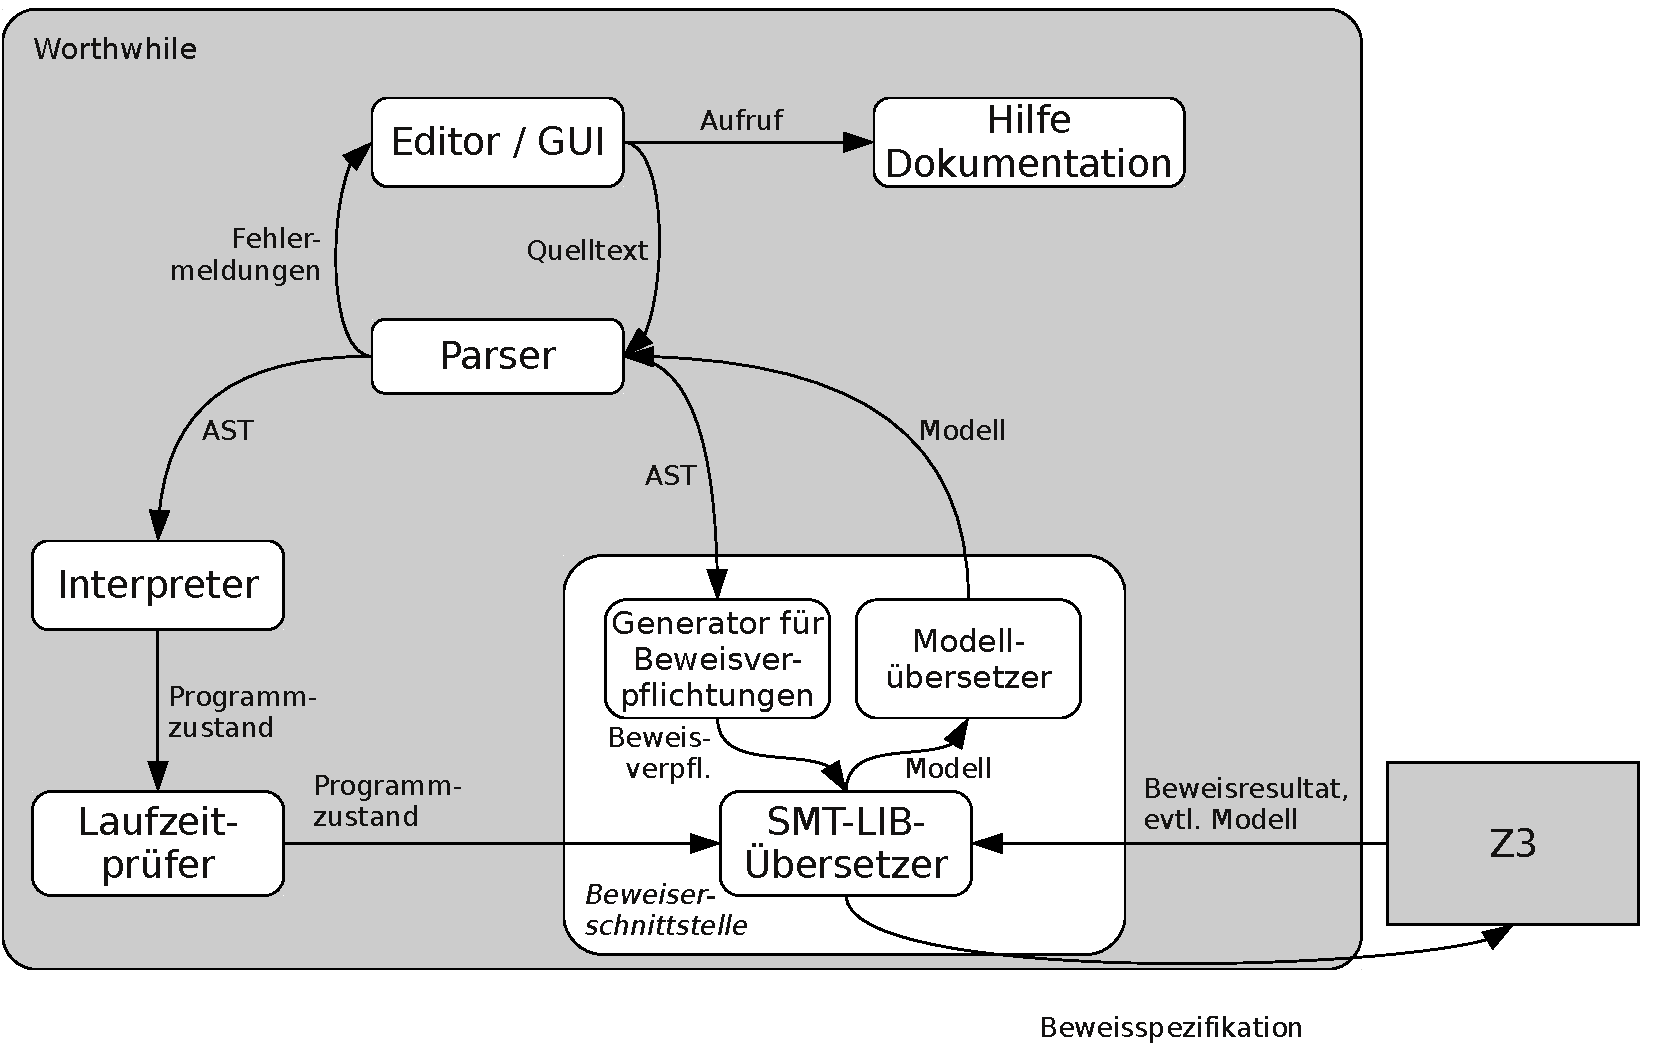
\includegraphics{architektur/architektur.pdf}


\section{Benutzeroberfläche}%

\subsection{Arbeitsumgebung}%

%\include{}

\subsection{Debugging}%

%\include{}


\section{Spezielle Anforderungen an die Entwicklungsumgebung}%

\begin{description}%
    \item [Teamkommunikation] Wiki (intern), E-Mail-Verteiler (intern)
    \item [Dokumentenerstellung] \see \LaTeX{}%
    \item [Entwurf] Ein Programm zur visualisierung der Programmstruktur
    \item [Versionskontrolle] \see Git%
    \item [Entwicklungsumgebung] \see Eclipse SDK, \see Eclipse Plug-in Development Environment, \see Xtext%
    \item [Validierung] Ein Testing Framework, um eine Test-Driven-Development-ähnliche Vorgehensweise bei der Entwicklung zu fördern
\end{description}%


\section{Zeit- und Ressourcenplanung}%

\subsection{Zeitaufwand}%

%\begin{left}
  \begin{tabular}{| l | l | l | }
    \hline
    zu implementierendes Modul & Zeitaufwand & Personen \\ \hline
    Parser &  &  \\ \hline
    Interpreter &  &  \\ \hline
    Laufzeitprüfer &  &  \\ \hline
    Schnittstelle zum Beweiser &  &  \\ \hline
    Grafische Benutzeroberfläche &  &  \\ \hline
    Dokumentation &  &  \\ \hline
    Beispielsammlung &  &  \\ \hline
    \hline
  \end{tabular}
%\end{center}

Die gesamte zur Verfügung stehende Implementierungszeit beträgt geschätzte 290 Arbeitsstunden pro Person, insgesamt also 1740 Personenarbeitsstunden.

\subsection{Phasenverantwortliche}%

%\begin{left}
  \begin{tabular}{| l | l | }
    \hline
    Phase & Verantwortlicher \\ \hline
    Pflichtenheft & Chris Hiatt \\ \hline
    Entwurf & ? \\ \hline
    Implementierung & ?,? \\ \hline
    Qualitätssicherung & ? \\ \hline
    Abnahme / Abschlusspräsentation & ? \\ \hline
    \hline
  \end{tabular}
%\end{center}

\subsection{Ressourcen}%

\begin{itemize}%
    \item Rechner,der die Mindestanforderungen erfüllt
\end{itemize}%


